\chapter{Track Simulation}
	In order to develop and test the~reconstruction algorithm, electron and positron tracks are simulated inside our detector with different initial parameters. Three approaches are used to simulate tracks for different purposes.
	
	The \textbf{Microscopic Simulation} uses the~Garfield++ toolkit~\cite{Garfield++}. Within this toolkit, the~program HEED (High Energy Electro-Dynamics)~\cite{HEED} is used to simulate the~primary particle and class \textit{AvalancheMicroscopic} to simulate the~drift of secondary electrons created by ionization in the gas. This is the most precise and time-consuming simulation used, our current goal is to be able to successfully reconstruct its results and determine our best-case energy resolution.
	
	The \textbf{Runge-Kutta Simulation} uses the 4th order Runge-Kutta numerical integration (\textcolor{red}{add citation for Runge-Kutta}) to simulate the~trajectory of the~primary particle in the~electromagnetic field inside the~detector. It is relatively fast since it does not simulate the secondary particles. It is used as a~part of our reconstruction algorithm as well as for testing of some parts of the reconstruction.
	
	The \textbf{Fast Simulation with Ionization Electron Map} is planned for the future, it will use the~HEED program~\cite{HEED} to simulate the~primary particle and the~Ionization Electron Map (see section~\ref{sec:map}) to simulate the~drift of secondary electrons. It should be significantly faster than the~Microscopic Simulation but offer comparable precision since it will rely on an already simulated drift map.
	
	All of these simulations require the~knowledge of the~electromagnetic field inside the~detector. Uniform electric field 400~V$\cdot$cm$^{-1}$ is assumed. The~magnetic field was simulated in Maxwell (\textcolor{red}{add citation? details? own subsection with figures? more details in section~\ref{sec:IEAP}?}).
	
	\textcolor{red}{Single track in positive x direction or initial parameters randomization. Importance of gas composition, used gas compositions.}
	
	\section{Microscopic Simulation}
		\textcolor{red}{Primary track simulated in HEED. Ionization electron drift simulated with AvalancheMicroscopic in Garfield.}
		
		\begin{figure}
			\centering
			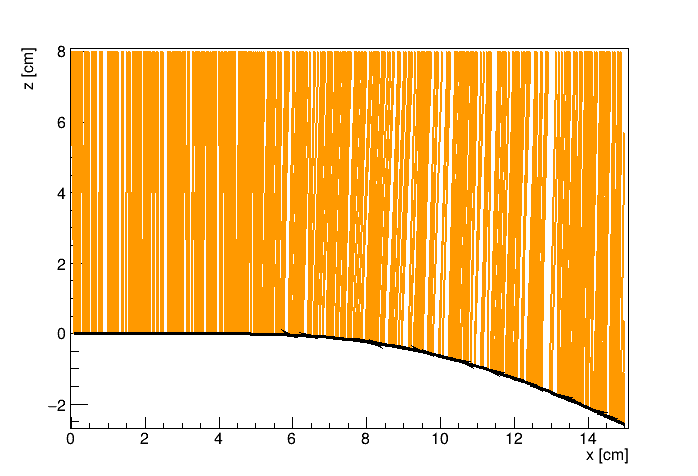
\includegraphics[width=0.3\textwidth]{7030_xz.png}
			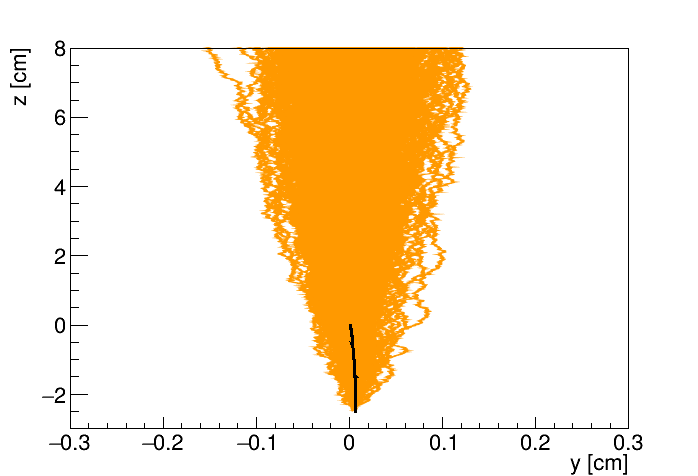
\includegraphics[width=0.3\textwidth]{7030_yz.png}
			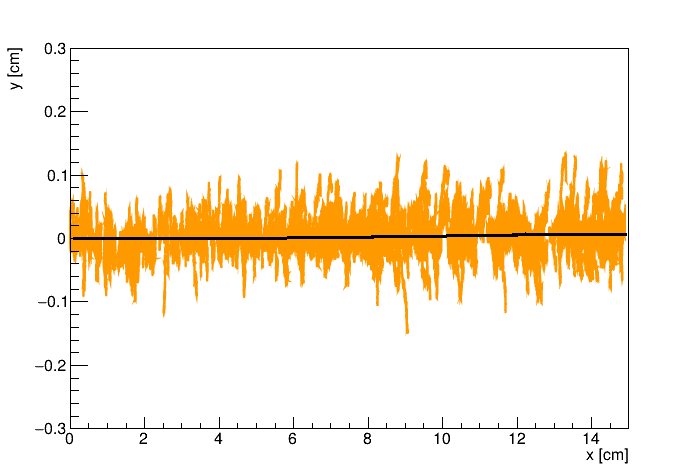
\includegraphics[width=0.3\textwidth]{7030_xy.png}
			\caption{Example of a~simulated electron track in 70~\%~argon and 30~\%~CO$_2$ atmosphere (on the left). \textcolor{red}{Swap for better images, better zoom. Explain drift lines, primary particle.}}
			\label{fig:7030sim}
		\end{figure}
		
		\begin{figure}
			\centering
			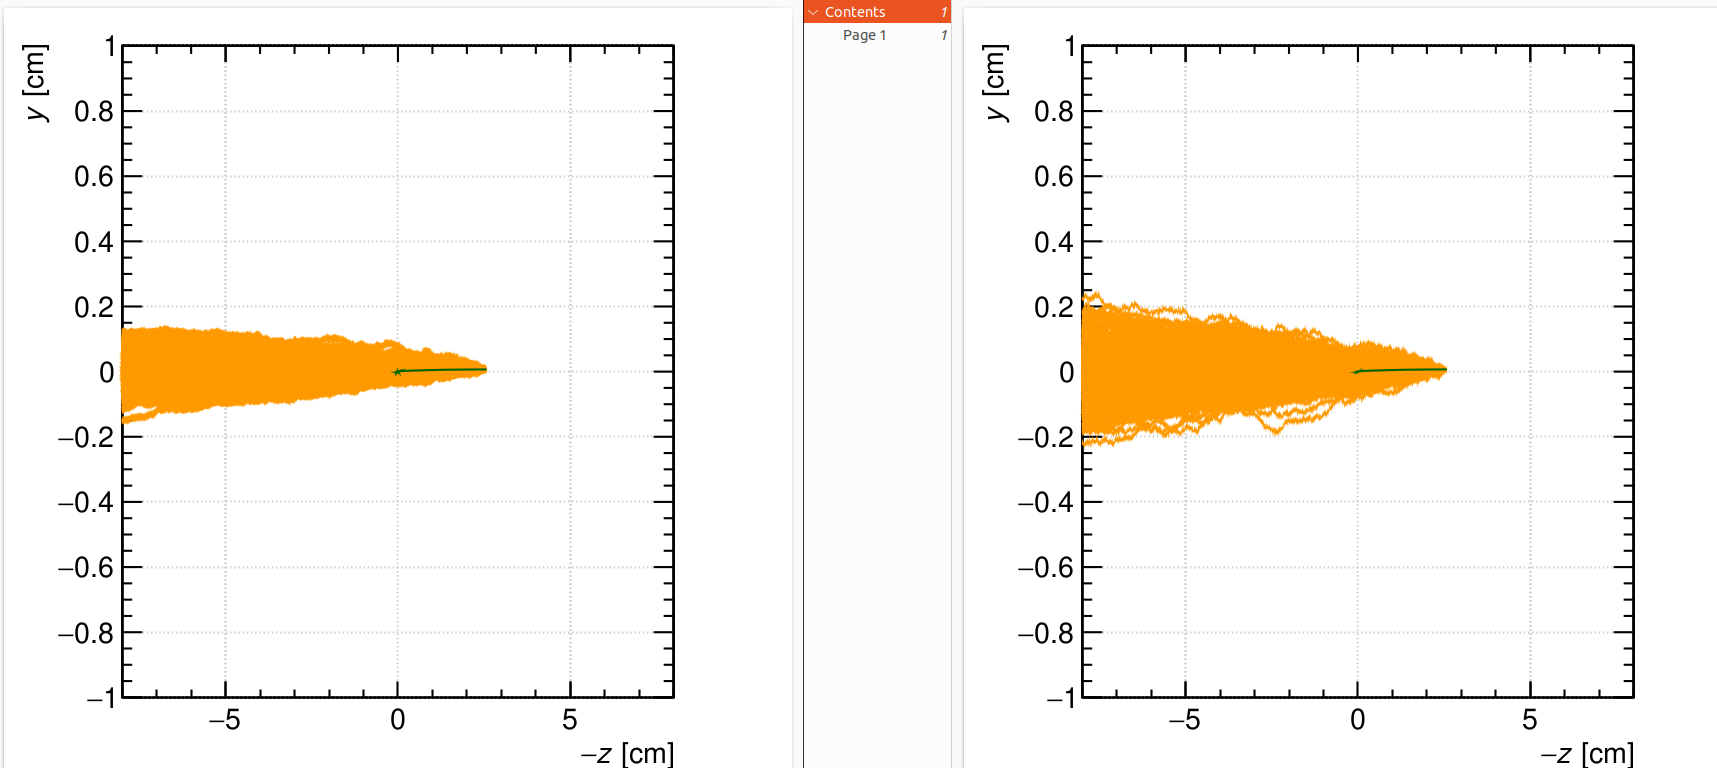
\includegraphics[width=0.9\textwidth]{diff_comp.png}
			\caption{Comparison of diffusion in a~simulated electron track in 70~\%~argon, 30~\%~CO$_2$ atmosphere and in 90~\%~argon, 10~\%~CO$_2$ atmosphere (on the right). \textcolor{red}{Swap for better image, better zoom. Or put same pictures for both comparisons in one subfigure, etc. Describe better.}}
			\label{fig:diffcomp}
		\end{figure}
	
	\section{Runge-Kutta Simulation}
	\label{sec:rks}
		\textcolor{red}{Trajectory simulation with 4th order Runge-Kutta. Relativistic equation that is numerically integrated by the algorithm.}
	
	\section{Future?: Fast Simulation with the Ionization Electron Map}
		\textcolor{red}{Primary track simulated in HEED. Readout parameters by interpolating the map. Diffusion from the map for randomization.}